% This LaTeX document needs to be compiled with XeLaTeX.
\documentclass[10pt]{article}
\usepackage[utf8]{inputenc}
\usepackage{ucharclasses}
\usepackage{amsmath}
\usepackage{amsfonts}
\usepackage{amssymb}
\usepackage[version=4]{mhchem}
\usepackage{stmaryrd}
\usepackage{bbold}
\usepackage{multirow}
\usepackage{graphicx}
\usepackage[export]{adjustbox}
\graphicspath{ {./images/} }
\usepackage{caption}
\usepackage{hyperref}
\hypersetup{colorlinks=true, linkcolor=blue, filecolor=magenta, urlcolor=cyan,}
\urlstyle{same}
\usepackage[fallback]{xeCJK}
\usepackage{polyglossia}
\usepackage{fontspec}
\usepackage{newunicodechar}
\IfFontExistsTF{Noto Serif CJK JP}
{\setCJKmainfont{Noto Serif CJK JP}}
{\IfFontExistsTF{STSong}
  {\setCJKmainfont{STSong}}
  {\IfFontExistsTF{Droid Sans Fallback}
    {\setCJKmainfont{Droid Sans Fallback}}
    {\setCJKmainfont{SimSun}}
}}
\IfFontExistsTF{Noto Serif CJK KR}
{\setCJKfallbackfamilyfont{\CJKrmdefault}{Noto Serif CJK KR}}
{\IfFontExistsTF{Apple SD Gothic Neo}
  {\setCJKfallbackfamilyfont{\CJKrmdefault}{Apple SD Gothic Neo}}
  {\IfFontExistsTF{UnDotum}
    {\setCJKfallbackfamilyfont{\CJKrmdefault}{UnDotum}}
    {\setCJKfallbackfamilyfont{\CJKrmdefault}{Malgun Gothic}}
}}

\setmainlanguage{english}
\setotherlanguages{greek}
\IfFontExistsTF{CMU Serif}
{\newfontfamily\lgcfont{CMU Serif}}
{\IfFontExistsTF{DejaVu Sans}
  {\newfontfamily\lgcfont{DejaVu Sans}}
  {\newfontfamily\lgcfont{Georgia}}
}
\setDefaultTransitions{\lgcfont}{}

\title{Identify latent group structures in panel data: The classifylasso command }

\author{Lingyun Zhou\\
Tsinghua University\\
Beijing, China\\
zhouly.23@pbcsf.tsinghua.edu.cn}
\date{}


\begin{document}
\maketitle
\captionsetup{singlelinecheck=false}


\begin{abstract}
In this article, we introduce a new command, classifylasso, that implements the classifier-lasso method (Su, Shi, and Phillips, 2016, Econometrica 84: 2215-2264) to simultaneously identify and estimate unobserved parameter heterogeneity in panel-data models using penalized techniques. We document the functionality of this command, including 1) penalized least-squares estimation of group-specific coefficients and classification of unknown group membership under a certain number of groups; 2) two lasso-type estimators with robust standard errors, namely, classifier-lasso and postlasso; and 3) determination of the number of groups based on an information criterion. We further develop some postestimation commands to display and visualize the estimation results.
\end{abstract}

Keywords: st0739, classifylasso, classifylasso postestimation, classoselect, classocoef, classogroup, unobserved parameter heterogeneity, latent group structures, classifier-lasso, penalized least squares, classification

\section*{1 Introduction}
Unobserved parameter heterogeneity has received increasing attention in both econometric theory and empirical studies (for example, Bonhomme and Manresa [2015]; Su, Shi, and Phillips [2016]; Eicher and Leukert [2009]; and Campello, Galvao, and Juhl [2019]). Conventional panel-data models assume either common slope coefficients or complete heterogeneity to facilitate estimation and inference. But validating these assumptions requires prior knowledge of economic models, which is most likely unavailable or unknowable to researchers. Therefore, recent theoretical works focus on unobserved parameter heterogeneity of unknown extent. Panel-data models with latent group structures where parameters are homogeneous within a group and heterogeneous across groups stand out. Two main approaches have been proposed to detect such group structures in panel-data models, namely, the clustering algorithm and the shrinkage method (for clustering algorithms, see Phillips and Sul [2007]; Bonhomme and Manresa [2015]; Sarafidis and Weber [2015]; and Carter, Schnepel, and Steigerwald [2017]; for\\[0pt]
shrinkage methods, see Su, Shi, and Phillips [2016]; Qian and Su [2016]; and Huang, Jin, and Su [2020]).

Several community-contributed commands deal with unobserved heterogeneity in different dimensions for empirical use. For instance, Bersvendsen and Ditzen (2021) introduce the xthst command to test slope heterogeneity; Lee and Steigerwald (2018), Du (2017), and Christodoulou and Sarafidis (2017) provide commands or packages like xtregcluster, clusteff, and psecta to study clustered data with latent group structures. However, all of these commands rely on clustering algorithms, such as the kmeans algorithm, and are sensitive to the initial partition and iterative process. We take the initiative to design a new command based on shrinkage techniques, namely, the classifierlasso (c-lasso) method, to fill the blank of latent group identification and estimation in Stata. This method is available in MATLAB and R (Gao and Shi 2021).

In this article, we illustrate how to fit panel-data models with latent group structures using Su, Shi, and Phillips's (2016) novel c-lasso estimation method using a new command, classifylasso, that is developed for the Stata environment. The c-lasso method simultaneously identifies and estimates unobserved slope heterogeneity in paneldata models without preassuming any explicit group structures. The core of the c-lasso method is to minimize a penalized objective function that combines an additive multiplication penalized term with the conventional least-squares function. The command classifylasso generates two lasso-type estimators, the c-lasso and postlasso estimators, which enjoy good theoretical properties. Additionally, when the number of groups is unknown, an information criterion is provided to select the number of groups consistently. The practitioners can either select the number of groups using the built-in option provided or determine the number of groups under the guidance of economic theories and treat it as an input. Simulation results show good finite-sample performance of the estimation results generated by classifylasso, which is compatible with the theoretical results in Su, Shi, and Phillips (2016).

We further provide a collection of postestimation commands to display and visualize the estimation results. Specifically, classoselect determines the active result; predict generates new variables containing group membership, fitted values, and residuals; estimates replay displays and exports the coefficient table; classocoef visualizes the coefficients in graphs; and classogroup plots the group selection information. The implementation of these postestimation commands are illustrated in an empirical replication of Su, Shi, and Phillips (2016) and an application motivated by Acemoglu et al. (2019).

The remainder of this article is organized as follows. Section 2 lays out the econometric framework and describes the estimation procedure. Section 3 presents details of the classifylasso command, and section 4 introduces the postestimation commands. Section 5 reports Monte Carlo simulation results. Section 6 empirically studies the potential unobserved group heterogeneity in the relationship between democracy and economic growth using the classifylasso command and compares the results with Acemoglu et al. (2019). Section 7 concludes.

\section*{2 Econometric framework}
In this section, we lay out the econometric framework of panel-data models with latent group structures and discuss the estimation procedure.

\subsection*{2.1 Panel-data models with latent group structures}
Consider the linear panel-data model


\begin{equation*}
y_{i t}=\mu_{i}+\boldsymbol{\beta}_{i}^{\prime} \mathbf{x}_{i t}+u_{i t}, \quad \text { for } \quad i=1,2, \ldots, N, \quad t=1,2, \ldots, T \tag{1}
\end{equation*}


where $y_{i t}$ is the dependent variable, $\mathbf{x}_{i t}$ is a $p \times 1$ vector of independent variables, $u_{i t}$ is the idiosyncratic error term with zero mean, and $\mu_{i}$ is the individual fixed effect. We further denote $\widetilde{y}_{i t}$ and $\widetilde{\mathbf{x}}_{i t}$ as the dependent and independent variables after concentrating out the fixed effects.

Our main interest is the $p \times 1$ vector of slope parameters, $\boldsymbol{\beta}_{i}$, which is assumed to follow an unknown group pattern as follows:

\[
\boldsymbol{\beta}_{i}= \begin{cases}\boldsymbol{\alpha}_{1}, & \text { if } i \in G_{1}  \tag{2}\\ \ldots & \ldots \\ \boldsymbol{\alpha}_{K}, & \text { if } i \in G_{K}\end{cases}
\]

$K$ is the number of latent groups, $\boldsymbol{\alpha}_{k}$ denotes the vector of slope parameters of the $k$ th group satisfying $\boldsymbol{\alpha}_{j} \neq \boldsymbol{\alpha}_{k}, j \neq k$, and $G_{k}$ denotes the set of members in group $k$ satisfying $\cup_{k=1}^{K} G_{k}=\{1, \ldots, N\}$ and $G_{j} \cap G_{k}=\emptyset$. That is, the coefficients are heterogeneous across groups and homogeneous within a group.

Let $\boldsymbol{\alpha}=\left(\boldsymbol{\alpha}_{1}^{\prime}, \ldots, \boldsymbol{\alpha}_{K}^{\prime}\right)^{\prime}$ and $\boldsymbol{\beta}=\left(\boldsymbol{\beta}_{1}^{\prime}, \ldots, \boldsymbol{\beta}_{N}^{\prime}\right)^{\prime}$. A penalized least-squares (PLS) objective function is developed to consistently estimate $\boldsymbol{\alpha}, \boldsymbol{\beta}$, and the group membership $G_{k}$ 's.

Before proceeding to the methodology, we emphasize several important assumptions required to achieve good theoretical properties of the estimators. First, both $N$ and $T$ are assumed to be large. Second, each group is assumed to have an asymptotically nonnegligible number of individuals, that is, $N_{k} / N \rightarrow \tau_{k} \in(0,1)$, where $N_{k}=\sum_{i=1}^{N} \mathbf{1}\left\{i \in G_{k}\right\}$ is the number of panel units in group $G_{k}$.

Moreover, the group-specific parameters satisfy the "beta-min" assumption, which states that $\min _{1 \leq k<l \leq K}\left\|\boldsymbol{\alpha}_{k}-\boldsymbol{\alpha}_{l}\right\| \geq c_{\alpha}>0$. This assumption indicates that the true coefficients are significantly different across the groups. Leeb and Pötscher (2005, 2006) and Pötscher and Leeb (2009) provide theoretical explanations on the inconsistency and nonnormal distribution of postselection estimators in the absence of the beta-min assumption. Simulation studies, such as the one by Drukker and Liu (2022) using nonlinear lasso models, further demonstrate the importance of this assumption. Belloni, Chernozhukov, and Hansen (2014) and Chernozhukov et al. (2018) discuss postselection estimators that do not require a beta-min assumption, resulting in a shift toward not imposing such an assumption. Recently, several commands have been developed to\\
provide postselection estimators without necessitating the beta-min assumption, such as the dsregress, poregress, and xporegress commands for linear models, along with their counterparts for logit and exponential mean models. Additionally, communitycontributed packages offering causal inference without the beta-min assumption can be found in Ahrens, Hansen, and Schaffer (2020), Ahrens et al. (2024), Drukker and Liu (2023), Drukker and Liu (Forthcoming), and Hirukawa et al. (2023).

The assumptions above ensure uniform classification consistency in large samples and thus the asymptotic behavior of the c-lasso and postlasso estimators. Other regularity conditions are omitted because of the space limitation; see Su, Shi, and Phillips (2016) for a detailed discussion.

\subsection*{2.2 Penalized least-squares estimation}
We follow a three-step procedure to estimate $\boldsymbol{\alpha}$. First, we construct a PLS objective function and obtain the c-lasso estimator given a fixed number of groups. Second, we obtain the postlasso estimator to achieve inference results and conduct bias corrections if needed given the estimated group membership. Lastly, an information criterion is constructed to determine the number of groups. The details are as follows:

Step 1. (C-lasso estimation) Given the number of groups $K$, the PLS objective function is constructed as


\begin{equation*}
Q_{N T, \lambda}^{(K)}=\frac{1}{N T} \sum_{i=1}^{N} \sum_{t=1}^{T}\left(\widetilde{y}_{i t}-\boldsymbol{\beta}_{i}^{\prime} \widetilde{\mathbf{x}}_{i t}\right)^{2}+\frac{\lambda_{N T}}{N} \sum_{i=1}^{N} \prod_{k=1}^{K}\left\|\boldsymbol{\beta}_{i}-\boldsymbol{\alpha}_{k}\right\| \tag{3}
\end{equation*}


where $\lambda_{N T}$ is a tuning parameter. The penalty term is a novel mixed additive multiplication form that shrinks the parameters of similar individuals to the same group. The c-lasso estimators $\widehat{\boldsymbol{\alpha}}=\left(\widehat{\boldsymbol{\alpha}}_{1}, \ldots, \widehat{\boldsymbol{\alpha}}_{K}\right)$ and $\widehat{\boldsymbol{\beta}}=\left(\widehat{\boldsymbol{\beta}}_{1}, \ldots, \widehat{\boldsymbol{\beta}}_{N}\right)$ are obtained by minimizing the above objective function; see (3). The membership of group $k$ is then given by

$$
\widehat{G}_{k}=\left\{i \in\{1,2, \ldots, N\}: \widehat{\boldsymbol{\beta}}_{i}=\widehat{\boldsymbol{\alpha}}_{k}\right\}, \quad k=1, \ldots, K
$$

According to assumption A2(i) in Su, Shi, and Phillips (2016), the tuning parameter $\lambda_{N T}$ should satisfy $T \lambda_{N T} /(\ln T)^{6+2 v} \rightarrow \infty$ and $\lambda_{N T}(\ln T)^{v} \rightarrow 0$ for some $v>0$ as $(N, T) \rightarrow \infty$. The conditions hold if $\lambda_{N T} \propto T^{-\alpha}$ for any $\alpha \in(0,1 / 2)$. In our command, we set $\lambda_{N T}=c_{\lambda} T^{-1 / 3}$ with a default $c_{\lambda}=0.2$. The simulation results in Su , Shi, and Phillips (2016) are robust when $c_{\lambda}=\{0.1,0.2,0.4,0.8,1.6\}$.

Because the objective function in (3) is not convex in $\boldsymbol{\beta}$, a numerical algorithm is developed to calculate the estimation result; see details in section 2.3.

Step 2. (Postlasso estimation) Given the estimated group results in step 1, the following postlasso estimators can be obtained:

$$
\widehat{\boldsymbol{\alpha}}_{\widehat{G}_{k}}=\left(\sum_{i \in \widehat{G}_{k}} \sum_{t=1}^{T} \widetilde{\mathbf{x}}_{i t} \widetilde{\mathbf{x}}_{i t}^{\prime}\right)^{-1} \sum_{i \in \widehat{G}_{k}} \sum_{t=1}^{T} \widetilde{\mathbf{x}}_{i t} \widetilde{y}_{i t}
$$

The c-lasso and postlasso estimators obtained from steps 1 and 2 have the asymptotic properties

$$
\begin{aligned}
\sqrt{N_{k} T}\left(\widehat{\boldsymbol{\alpha}}_{k}-\boldsymbol{\alpha}_{k}\right)-\overline{\boldsymbol{\Phi}}_{k}^{-1} \boldsymbol{\theta}_{k N T} \xrightarrow[N, T \rightarrow \infty]{D} N\left(0, \boldsymbol{\Phi}_{k}^{-1} \boldsymbol{\Psi}_{k} \boldsymbol{\Phi}_{k}^{-1}\right), & k=1, \ldots, K \\
\sqrt{N_{k} T}\left(\widehat{\boldsymbol{\alpha}}_{\widehat{G}_{k}}-\boldsymbol{\alpha}_{k}\right)-\overline{\boldsymbol{\Phi}}_{k}^{-1} \boldsymbol{\theta}_{k N T} \xrightarrow[N, T \rightarrow \infty]{D} N\left(0, \boldsymbol{\Phi}_{k}^{-1} \boldsymbol{\Psi}_{k} \boldsymbol{\Phi}_{k}^{-1}\right), & k=1, \ldots, K
\end{aligned}
$$

where $\overline{\boldsymbol{\Phi}}_{k}=1 /\left(N_{k} T\right) \sum_{i \in G_{k}} \sum_{t=1}^{T} \widetilde{\mathbf{x}}_{i t} \widetilde{\mathbf{x}}_{i t}^{\prime} \xrightarrow{P} \boldsymbol{\Phi}_{k}>0$, $\boldsymbol{\theta}_{k N T}=1 / \sqrt{N_{k} T} \sum_{i \in G_{k}} \sum_{t=1}^{T} \mathbb{E}\left(\mathbf{x}_{i t} \widetilde{u}_{i t}\right)$, and $\boldsymbol{\Psi}_{k}=\lim _{T \rightarrow \infty} 1 / T \sum_{t=1}^{T} \sum_{s=1}^{T} \mathbb{E}\left(\mathbf{x}_{i t} \mathbf{x}_{i s}^{\prime} u_{i t} u_{i s}\right)$.

The above consistency results strongly rely on the beta-min assumption. In other words, if the group-specific coefficients are different but not distinct enough, many individuals will be inaccurately classified, leading to inconsistent estimation results. In section 5 , we discuss the violation of beta-min assumption numerically.

The term $\overline{\boldsymbol{\Phi}}_{k}^{-1} \boldsymbol{\theta}_{k N T}$ is also critical to the consistency of $\widehat{\boldsymbol{\alpha}}$. For example, in the static panels, we presume that $\mathbf{x}_{i t}$ is strictly exogenous, so $\boldsymbol{\theta}_{k N T}=o_{P}(1)$ and $\widehat{\boldsymbol{\alpha}}$ are consistent. However, in the dynamic panels, $\mathbf{x}_{i t}$ contains lagged dependent variables, so $\widehat{\boldsymbol{\alpha}}$ is inconsistent. In the latter case, we correct the estimation bias through Dhaene and Jochmans's (2015) half-panel jackknife method.

The theoretical results in Su, Shi, and Phillips (2016) indicate that $\widehat{\boldsymbol{\alpha}}_{k}$ and $\widehat{\boldsymbol{\alpha}}_{\widehat{G}_{k}}$ are asymptotically equivalent and both enjoy the oracle property. Despite this, in practice the postlasso estimator is commonly favored over the c-lasso estimator because of its superior performance in finite samples, as well as its beneficial smaller bias (as also noted in remark 4 by Su, Shi, and Phillips [2016] and Belloni and Chernozhukov [2013]). Consequently, we advise users to rely primarily on postlasso estimates. We have set the postlasso estimates as the default display in the command and also present these estimates in the subsequent simulation and empirical studies.

Step 3. (Determination of the number of groups) In practice, the number of groups $K$ might be unknown. Replacing $K$ in (3) with $\widehat{K}$, we allow the dependency of $\widehat{\boldsymbol{\alpha}}, \widehat{\boldsymbol{\beta}}$, and $\widehat{G}_{k}$ on $\widehat{K}$ and $\lambda$ such that $\widehat{\boldsymbol{\alpha}}=\widehat{\boldsymbol{\alpha}}(\widehat{K}, \lambda), \widehat{\boldsymbol{\beta}}=\widehat{\boldsymbol{\beta}}(\widehat{K}, \lambda)$, and $\widehat{G}_{k}=\widehat{G}_{k}(\widehat{K}, \lambda)$, and we obtain the postlasso estimator as $\widehat{\alpha}_{\widehat{G}_{k}(\widehat{K}, \lambda)}$. Then the number of groups can be obtained by minimizing the information criterion


\begin{equation*}
\operatorname{IC}(\widehat{K}, \lambda)=\ln \left(\widehat{\sigma}_{\widehat{G}(\widehat{K}, \lambda)}^{2}\right)+\rho_{N T} p \widehat{K} \tag{4}
\end{equation*}


where $\widehat{\sigma}_{\widehat{G}(\widehat{K}, \lambda)}^{2}=1 /(N T) \sum_{k=1}^{\widehat{K}} \sum_{i \in \widehat{G}_{k}(\widehat{K}, \lambda)} \sum_{t=1}^{T}\left(\widetilde{y}_{i t}-\widehat{\boldsymbol{\alpha}}_{\widehat{G}_{k}(\widehat{K}, \lambda)}^{\prime} \widetilde{\mathbf{x}}_{i t}\right)^{2}$ and $\rho_{N T}$ is the tuning parameter. Su, Shi, and Phillips (2016) demonstrate that with the beta-min assumption and a proper convergence rate of the tuning parameter, the information criterion determines the correct number of groups with probability approaching 1 (w.p.a.1).

According to assumption A5* in Su, Shi, and Phillips (2016), in the case of linear models, the tuning parameter $\rho_{N T}$ should satisfy $\rho_{N T} \rightarrow 0$ and $\rho_{N T} \delta_{N T}^{2} \rightarrow \infty$, where\\
$\delta_{N T}=N^{1 / 2} T^{1 / 2}$ if $x_{i t}$ is exogenous and $\min \left(N^{1 / 2} T^{1 / 2}, T\right)$ otherwise. Monte Carlo simulations in Su, Shi, and Phillips (2016) and Lu and Su (2017) both indicate that $\rho_{N T}=c_{\rho}(N T)^{-1 / 2}$ with $c_{\rho}=2 / 3$ works well in the linear models.

\subsection*{2.3 Iterative algorithm}
We now introduce the numerical algorithm to be used in the aforementioned step 1 in section 2.2.\\
Step 1.1. (Initial estimates) The classifylasso command starts with initial $\widehat{\boldsymbol{\alpha}}^{(0)}= \left(\boldsymbol{\alpha}_{1}^{(0) \prime}, \ldots, \widehat{\boldsymbol{\alpha}}_{K}^{(0) \prime}\right)^{\prime}=\mathbf{0}_{p K \times 1}$ and $\widehat{\boldsymbol{\beta}}^{(0)}=\left(\widehat{\boldsymbol{\beta}}_{1}^{(0) \prime}, \ldots, \widehat{\boldsymbol{\beta}}_{N}^{(0) \prime}\right)^{\prime}$. Here $\mathbf{0}_{p K \times 1}$ denotes a $p K \times 1$ zero matrix, and

$$
\widehat{\boldsymbol{\beta}}_{i}^{(0)}= \begin{cases}\left(\mathbf{X}_{i}^{\prime} \mathbf{X}_{i}\right)^{-1} \mathbf{X}_{i}^{\prime} \mathbf{y}_{i}, & \text { if } \mathbf{y}_{i}^{\prime} \mathbf{y}_{i}>0.0001 N \\ \left(\mathbf{X}^{\prime} \mathbf{X}\right)^{-1} \mathbf{X}^{\prime} \mathbf{y}, & \text { if } \mathbf{y}_{i}^{\prime} \mathbf{y}_{i} \leq 0.0001 N\end{cases}
$$

where $\mathbf{y}_{i}$ and $\mathbf{X}_{i}$ are a $T \times 1$ vector and a $T \times p$ matrix that denote the dependent and independent variables of individual $i$ and $\mathbf{X}=\left(\mathbf{X}_{1}^{\prime}, \ldots, \mathbf{X}_{N}^{\prime}\right)^{\prime}, \mathbf{y}=\left(\mathbf{y}_{1}^{\prime}, \ldots, \mathbf{y}_{N}^{\prime}\right)^{\prime}$. If the variation of the dependent variable of individual $i$ is large enough, the initial value is set to its time-series estimation result; otherwise, the pooled panel one is used.\\
Step 1.2. (Conditional minimization) Suppose we have obtained $\widehat{\boldsymbol{\alpha}}^{(r-1)}$ and $\widehat{\boldsymbol{\beta}}^{(r-1)}$ at the $r$ th iteration, $r \geq 1$. Let $Q_{N T}^{\mathrm{ols}}(\boldsymbol{\beta})=1 /(N T) \sum_{i=1}^{N} \sum_{t=1}^{T}\left(\widetilde{y}_{i t}-\boldsymbol{\beta}_{i}^{\prime} \widetilde{\mathbf{x}}_{i t}\right)^{2}$, and

$$
\left\{\begin{array}{l}
\left(\widehat{\boldsymbol{\beta}}^{(r, 1)}, \widehat{\boldsymbol{\alpha}}_{1}^{(r)}\right)=\underset{\boldsymbol{\beta}, \boldsymbol{\alpha}_{1}}{\arg \min }\left(Q_{N T}^{\mathrm{ols}}(\boldsymbol{\beta})+\frac{\lambda}{N} \sum_{i=1}^{N}\left\|\boldsymbol{\beta}_{i}-\boldsymbol{\alpha}_{1}\right\| \prod_{k \neq 1}^{K}\left\|\widehat{\boldsymbol{\beta}}_{i}^{(r-1)}-\widehat{\boldsymbol{\alpha}}_{k}^{(r-1)}\right\|\right) \\
\left(\widehat{\boldsymbol{\beta}}^{(r, 2)}, \widehat{\boldsymbol{\alpha}}_{2}^{(r)}\right)=\underset{\boldsymbol{\beta}, \boldsymbol{\alpha}_{2}}{\arg \min }\left(Q_{N T}^{\mathrm{ols}}(\boldsymbol{\beta})+\frac{\lambda}{N} \sum_{i=1}^{N}\left\|\widehat{\boldsymbol{\beta}}_{i}^{(r, 1)}-\widehat{\boldsymbol{\alpha}}_{1}^{(r)}\right\|\left\|\boldsymbol{\beta}_{i}-\boldsymbol{\alpha}_{2}\right\| \prod_{k \neq 1,2}^{K}\left\|\widehat{\boldsymbol{\beta}}_{i}^{(r-1)}-\widehat{\boldsymbol{\alpha}}_{k}^{(r-1)}\right\|\right) \\
\cdots \cdots \\
\left(\widehat{\boldsymbol{\beta}}^{(r, K)}, \widehat{\boldsymbol{\alpha}}_{K}^{(r)}\right)=\underset{\boldsymbol{\beta}, \boldsymbol{\alpha}_{K}}{\arg \min }\left(Q_{N T}^{\mathrm{ols}}(\boldsymbol{\beta})+\frac{\lambda}{N} \sum_{i=1}^{N} \prod_{k=1}^{K-1}\left\|\widehat{\boldsymbol{\beta}}_{i}^{(r, k)}-\widehat{\boldsymbol{\alpha}}_{k}^{(r)}\right\|\left\|\boldsymbol{\beta}_{i}-\boldsymbol{\alpha}_{K}\right\|\right)
\end{array}\right.
$$

We hence obtain $\widehat{\boldsymbol{\alpha}}^{(r)}=\left(\widehat{\boldsymbol{\alpha}}_{1}^{(r)}, \ldots, \widehat{\boldsymbol{\alpha}}_{K}^{(r)}\right)$ and $\widehat{\boldsymbol{\beta}}^{(r)}=\widehat{\boldsymbol{\beta}}^{(r, K)}$.\\
Step 1.3. (Convergence criterion) The iterative algorithm ends if $r=R_{\text {max }}$ or


\begin{equation*}
\frac{\sum_{i=1}^{N}\left\|\widehat{\boldsymbol{\beta}}_{i}^{(r)}-\widehat{\boldsymbol{\beta}}_{i}^{(r-1)}\right\|}{\sum_{i=1}^{N}\left\|\widehat{\boldsymbol{\beta}}_{i}^{(r)}\right\|+0.0001}<\epsilon_{\mathrm{tol}} \text { and } \frac{\sum_{i=1}^{N}\left\|\widehat{\boldsymbol{\alpha}}_{i}^{(r)}-\widehat{\boldsymbol{\alpha}}_{i}^{(r-1)}\right\|}{\sum_{i=1}^{N}\left\|\widehat{\boldsymbol{\alpha}}_{i}^{(r)}\right\|+0.0001}<\epsilon_{\mathrm{tol}} \tag{5}
\end{equation*}


where $R_{\text {max }}$ is the maximum number of iterations and $\epsilon_{\text {tol }}$ is the tolerance level. Let $R$ be the largest number that meets the above criterion, so $\widehat{\boldsymbol{\beta}}=\widehat{\boldsymbol{\beta}}^{(R)}$ and $\widehat{\boldsymbol{\alpha}}=\widehat{\boldsymbol{\alpha}}^{(R)}$.

\section*{3 The classifylasso command}
The command classifylasso estimates (1)-(2) using the c-lasso and selects the number of groups according to (4). The command records the iteration process, displays\\
the estimation table, and stores results in e() form. Postestimation commands are designed to further manipulate these results; see section 4. This section documents the syntax and functionalities of the classifylasso command. The panel structure must be declared by xtset or tsset beforehand. Commands reghdfe (Correia 2014) and ftools (Correia 2016) are required to treat with fixed effects.

\subsection*{3.1 Syntax}
The syntax of the classifylasso command is as follows:

\begin{verbatim}
classifylasso depvar indepvars [if] [in] [, grouplist(numlist) lambda( \#)
    rho(\#) tolerance(\#) maxiterations(\#) optimize_options absorb(varlist)
    noabsorb vce(vcetype) dynamic notable display_options]
\end{verbatim}

where depvar is the dependent variable, that is, $y_{i t}$ in (1), and indepvar is a list of independent variables, that is, $\mathbf{x}_{i t}$ in (1).

\subsection*{3.2 Options}
grouplist(numlist) specifies the possible number (list) of latent groups, that is, $K$ in (2) or $\widehat{K}$ 's in (4). The default is grouplist(2).\\
lambda(\#) specifies the constant $c_{\lambda}$ in the tuning parameter $\lambda_{N T}=c_{\lambda} T^{-1 / 3}$ of the PLS objective function in (3). The default is lambda (0.2).\\
rho(\#) specifies the constant $c_{\rho}$ in the tuning parameter $\rho_{N T}=c_{\rho}(N T)^{-1 / 2}$ of the information criterion in (4). The default is rho(0.67).\\
tolerance (\#) specifies the tolerance criterion for convergence in the iterative algorithm, that is, $\epsilon_{\text {tol }}$ in (5). The default is tolerance(0.01).\\
maxiterations(\#) specifies the maximum level of iterations in the iterative algorithm, that is, $R_{\text {max }}$ in (5). The default is maxiterations(20).\\
optimize\_options control the optimize package. optptol(\#), optvtol(\#), optnrtol(\#), optmaxiter(\#), and optignorenrtol(string) determine the convergence criterion; their defaults are $1 \mathrm{e}-6,1 \mathrm{e}-7,1 \mathrm{e}-5,150$, and "off", respectively. opttechnique(string) and optsingularHmethod(string) determine the optimization algorithm and singular method; their defaults are "bfgs" and "m-marquardt", respectively. See [M-5] optimize() for more details.\\
absorb(varlist) specifies the categorical variables that identify the fixed effects; the default is to absorb the individual fixed effects identified by the panel (unit) variable.\\
noabsorb suppresses the fixed effects.\\[0pt]
vce(vcetype) specifies the standard error type in postlasso estimation, which includes types that are derived from asymptotic theory (ols, the default), that are robust to some kinds of misspecification (robust), and that allow for intragroup correlations (cluster clustvar); see [R] Estimation options.\\
dynamic applies Dhaene and Jochmans's (2015) half-panel jackknife method to conduct bias corrections in dynamic models.\\
notable suppresses the estimation table.\\
display\_options control the display style. They include noci, nopvalues, noomitted, vsquish, noemptycells, baselevels, allbaselevels, nofvlabel, fvwrap(\#), fvwrapon(style), cformat (\% fmt), pformat (\% fmt), sformat (\%fmt), and nolstretch; see $[\mathrm{R}]$ Estimation options.

\subsection*{3.3 Stored results}
classifylasso stores the following results in e():\\
Scalars\\
e (N)\\
e(obs)\\
e(group)\\
Macros\\
e(cmd)\\
e(cmdline)\\
e(depvar)\\
e(title)\\
e(predict)\\
e(panelvar)\\
e(timevar)\\
e(indepvar)\\
e(absvar)\\
e(grouplist)\\
e(coef)\\
Matrices\\
e(a\_classo\_GK)\\
e(V\_classo\_GK)\\
e(rsq\_classo\_GK)\\
e(a\_post\_GK)\\
e(V\_post\_GK)\\
e(rsq\_post\_GK)\\
e(df\_GK)\\
e(id)\\
e(selection)\\
Functions\\
e(sample)\\
number of individual units\\
sample size\\
selected number of groups\\
classifylasso\\
command as typed\\
name of dependent variable\\
Classifier-lasso\\
classifylasso\_p\\
name of panel variable\\
name of time variable\\
name of independent variables\\
name of the absorbed variables\\
possible group number list\\
active coefficients, postselection or penalized\\
c-lasso coefficient matrix under $K$ groups\\
c-lasso covariance matrix under $K$ groups\\
c-lasso $R^{2}$ under $K$ groups\\
postlasso coefficient matrix under $K$ groups\\
postlasso covariance matrix under $K$ groups\\
postlasso $R^{2}$ under $K$ groups\\
degrees of freedom under $K$ groups\\
group membership and individual information matrix\\
selection information matrix\\
marks estimation sample

\subsection*{3.4 Implementation example}
In what follows, we illustrate how to use the classifylasso command to implement estimation in Stata. We show the estimation process here and postpone the postesti-\\
mation part to section 4.6. The output of our command is the same as that in Su, Shi, and Phillips' (2016) empirical study of the determinants of savings through a balanced panel of 56 countries from 1995 to 2010.

The regression model is

$$
\operatorname{saving}_{i t}=\beta_{1 i} \operatorname{saving}_{i, t-1}+\beta_{2 i} \% \Delta \mathrm{CPI}_{i t}+\beta_{3 i} \text { interest }_{i t}+\beta_{4 i} \% \Delta \mathrm{GDP}_{i t}+\mu_{i}+u_{i t}
$$

where $i$ and $t$ denote the country and year indices; the dependent variable saving is the ratio of savings to gross domestic product (GDP); the independent variables include one lag of the dependent variable saving, consumer price index (CPI)-based inflation rate $\% \Delta \mathrm{CPI}$, real interest rate interest, and GDP growth rate $\% \Delta \mathrm{GDP} ; \mu_{i}$ is the individual fixed effect; $u_{i t}$ is the idiosyncratic error. The data used are stored in saving.dta, provided with the article files.

The following codes implement the c-lasso estimation. We first import the data and declare the panel and time variables. Then we use the classifylasso command to identify latent group structures. We follow Su, Shi, and Phillips (2016) to set the tuning parameter $c_{\lambda}=1.5485$, use the dynamic panel, and select the group numbers from 1 to 5.

\begin{verbatim}
- use saving
- xtset code year
Panel variable: code (strongly balanced)
    Time variable: year, 1 to 15
        Delta: 1 unit
. classifylasso savings lagsavings cpi interest gdp, grouplist(1/5)
> lambda(1.5485) tolerance(1e-4) dynamic
Estimation 1: Group Number = 1; Iteration: \sqrt{}{}
Information Criterion = -.359883766
Estimation 2: Group Number = 2; Iteration: 1 ..5 ...10...15...20 
Information Criterion = -.369981214
Estimation 3: Group Number = 3; Iteration: 1 ⋯ 5 ...10...15...20 
Information Criterion = -. }30227990
Estimation 4: Group Number = 4; Iteration: 1 ⋯ 5 ...10...15...20 
Information Criterion = -. }19803439
Estimation 5: Group Number = 5; Iteration: 1..5...10...15...20 
Information Criterion = -. }10647405
* Selected Group Number: 2
The algorithm takes 9min54s.
\end{verbatim}

\begin{center}
\begin{tabular}{|l|l|l|l|l|l|l|}
\hline
\multicolumn{3}{|l|}{Classifier-Lasso linear model} & \multirow{2}{*}{} & \multicolumn{2}{|r|}{Number of obs =} & 840 \\
\hline
\multicolumn{3}{|l|}{Postestimation with 2 groups} &  &  & Number of units = & 56 \\
\hline
\multicolumn{4}{|l|}{Fixed effect estimation with Group 1} & \multicolumn{2}{|r|}{R-squared =} & 0.4988 \\
\hline
\multicolumn{4}{|l|}{Absorbing: code} &  & Adj R-squared & 0.4592 \\
\hline
No. of obs = & \multicolumn{3}{|c|}{465} &  & Within R-sq. & 0.4988 \\
\hline
No. of units = & \multicolumn{3}{|c|}{31} & Root MSE & = & 0.7362 \\
\hline
savings & Coefficient & Std. err. & z & $\mathrm{P}>|\mathrm{z}|$ & [95\% conf. & interval] \\
\hline
lagsavings & . 6952103 & . 0383023 & 18.15 & 0.000 & . 6201392 & . 7702815 \\
\hline
cpi & -. 160168 & . 039182 & -4.09 & 0.000 & -. 2369634 & -. 0833727 \\
\hline
interest & -. 1490145 & . 0368407 & -4.04 & 0.000 & -. 221221 & -. 076808 \\
\hline
gdp & . 2892251 & . 0379408 & 7.62 & 0.000 & . 2148624 & . 3635878 \\
\hline
\_cons & . 0550013 & . 0320203 & 1.72 & 0.086 & -. 0077574 & . 11776 \\
\hline
\multicolumn{4}{|l|}{Fixed effect estimation with Group 2} & \multicolumn{2}{|r|}{R-squared =} & 0.4372 \\
\hline
\multicolumn{4}{|l|}{Absorbing: code} &  & Adj R-squared = & 0.3917 \\
\hline
No. of obs = & \multicolumn{3}{|c|}{375} & \multicolumn{2}{|r|}{Within R-sq. =} & 0.4372 \\
\hline
\multicolumn{4}{|l|}{\begin{tabular}{l}
No. of units = \\
25 \\
\end{tabular}} & \multicolumn{2}{|r|}{Root MSE =} & 0.7810 \\
\hline
savings & Coefficient & Std. err. & $z$ & $\mathrm{P}>|\mathrm{z}|$ & [95\% conf. & interval] \\
\hline
lagsavings & . 6938863 & . 0356796 & 19.45 & 0.000 & . 6239556 & . 763817 \\
\hline
cpi & . 1967192 & . 0399412 & 4.93 & 0.000 & . 1184359 & . 2750025 \\
\hline
interest & . 1225496 & . 0411717 & 2.98 & 0.003 & . 0418545 & . 2032447 \\
\hline
gdp & . 1126528 & . 0474176 & 2.38 & 0.018 & . 0197161 & . 2055896 \\
\hline
\_cons & -. 0067423 & . 0401331 & -0.17 & 0.867 & -. 0854018 & . 0719172 \\
\hline
\end{tabular}
\end{center}

Both the basic information and the iterative process are displayed. Each dot visualizes a complete iteration in step 1.2, as described in section 2.3. The information criterion suggests that the countries cluster into two latent groups. The two coefficient tables are then displayed. First, the coefficients of the inflation rate and the real interest rate become significant in both groups, albeit with opposite signs. Second, the coefficients of the GDP growth rate are significant at the $5 \%$ level in both groups, implying a positive correlation between savings rates and income growth across nations. For an extended discussion on this example, please refer to section 5.1 in Su, Shi, and Phillips (2016).

We apply the following codes to store the estimation results in ssp2016.ster. Users can manipulate these results using the postestimation commands as described in section 4 . Examples of this are presented in section 4.6.

\begin{verbatim}
. estimates save ssp2016
file ssp2016.ster saved
\end{verbatim}

\section*{4 The postestimation commands}
We give five postestimation commands-classoselect, predict, estimates replay, classocoef, and classogroup - to select active estimation results, generate new variables, display coefficient tables, and visualize the results after executing classifylasso. The introduction and examples are as follows.

\subsection*{4.1 The classoselect command}
The classoselect command decides an alternative estimation result to be used in the following predict, estimates replay, and classocoef commands. It chooses the number of groups and whether the c-lasso or postlasso estimates are used. By default, postlasso coefficients with the information criterion-best number of groups are selected.

\subsection*{4.1.1 Syntax and options}
\begin{verbatim}
classoselect [, group(#) postselection penalized]
\end{verbatim}

group (\#) specifies the number of groups used to estimate the coefficients. This number must be included in the list specified by grouplist() in classifylasso.\\
postselection specifies that postlasso coefficients be used to plot the graph. That is the default. Postlasso coefficients are calculated by regressing the corresponding model for each estimated group.\\
penalized specifies that penalized coefficients be used to plot the graph. Penalized coefficients are those estimated by c-lasso in the calculation of the additive multiplication penalty.

\subsection*{4.2 The predict command}
predict helps users to generate new variables containing the group membership and fitted values from the active estimation results selected by classoselect.

\subsection*{4.2.1 Syntax and options}
predict newvar [if] [in] [, statistic]\\
gid predicts the group membership, and it is the default.\\
$\mathrm{xb}, \mathrm{xbd}, \mathrm{d}$, residuals, and $\underline{s} t d p$ calculate the linear prediction, fixed effects, sum of xb and d , deviation of xbd from the dependent variable, and the standard deviation of linear prediction. The predictions are analogous to reghdfe.

\subsection*{4.3 The estimates replay command}
The estimates command displays and exports the coefficient tables from the active estimation results selected by classoselect.

\subsection*{4.3.1 Syntax and options}
estimates replay [, outreg2(filename [, options]) display\_options]\\[0pt]
outreg2(filename[, options]) exports the coefficients to the local disk. Each group forms a column. Because e(b) and e(V) are not stored, this option is the only way to export tables. The default is not to export; see outreg2 (Wada 2005) for details.\\
display\_options control the display style; these options are the same as those in the command classifylasso.

\subsection*{4.4 The classocoef command}
The classocoef command uses graph twoway to visualize the coefficient estimates from the active estimation results selected by classoselect. The command generates graphs for all variables by default or for designated variables, with one variable per graph.

In each graph, the $y$ axis and $x$ axis indicate the value of the coefficient and the individual identity, respectively. There are four major elements: the group-specific coefficient line, the confidence interval lines, the scatters of individual-specific timeseries estimates, and the horizontal zero line. This command allows users to visualize one or more of these four elements.

\subsection*{4.4.1 Syntax and options}
classocoef [indepvars] [, global\_twoway\_options groupcoef\_line\_options groupci\_line\_options tscoef\_scatter\_options zero\_line\_options]\\
global\_twoway\_options specify how the overall style looks.\\
colors(string) specifies the color list for different groups. The default is colors("maroon dkorange sand forest\_green navy").\\[0pt]
title(tinfo), subtitle(tinfo), legend([contents] [location]), ytitle(axis\_title), xtitle(axis\_title), ylabel(rule\_or\_values), and xlabel(rule\_or\_values) control the corresponding titles, legends, and axis; see [G-3] title\_options, [G-3] legend\_options, and [G-3] axis\_options. The defaults are shown in the examples.\\[0pt]
name(name\_option), saving(saving\_option), export(name[,options]), and scheme(schemename) specify the graph name, the save path, the export name, and the overall look, respectively. Note that if there is more than one graph to be generated, modifying these options may cause an error.\\[0pt]
twoptions(twoway\_options) specifies additional two-way options; see [G-2] graph twoway.\\
nowindow suppresses the graph window.\\
groupcoef\_line\_options control the group-specific coefficient line, and nocoefplot suppresses the line.\\
coeflwidth(linewidthstyle) and coeflpattern(linepatternstyle) specify the line style. The default is coeflwidth(1) and coeflpattern(solid).\\[0pt]
coefoptions(line\_options) specifies additional line options; see [G-2] graph twoway line.\\
groupci\_line\_options control the confidence interval lines, and nociplot suppresses the lines.\\
level(\#) controls the significance level as classotable.\\
cilwidth(linewidthstyle) and cilpattern(linepatternstyle) specify the line style. The default is cilwidth(0.5) and cilpattern(dash).\\[0pt]
cioptions(line\_options) specifies additional line options; see [G-2] graph twoway line.\\
tscoef\_scatter\_options control the scatters of time-series estimates, and\\
notsscatter suppresses the scatters.\\
tsmsize(markersize) specifies the scatter size. The default is tsmsize(0.5).\\[0pt]
tsoptions(scatter\_options) specifies additional options; see [G-2] graph twoway scatter.\\
zero\_line\_options control the horizontal zero line, and nozeroline suppresses the line.\\
zerolwidth(linewidthstyle), zerolpattern(linepatternstyle), and zerolcolor(colorstyle) specify the line style. The defaults are zerolwidth(0.5), zerolpattern(solid), and zerolcolor(black).\\[0pt]
zerooptions(line\_options) specifies additional line options; see [G-2] graph twoway line.

\subsection*{4.5 The classogroup command}
The classogroup command uses graph twoway to visualize the group-number selection information. Both information criterion values and numbers of iterations are plotted, which are measured by $y$-axis(1) and $y$-axis(2), respectively. The $x$ axis indicates the group number. The selected number of groups is marked by a triangle.

\subsection*{4.5.1 Syntax and options}
\begin{verbatim}
classogroup [, global_twoway_options icplot_options iterplot_options]
global_twoway_options specify how the overall style looks.
    title(tinfo), subtitle(tinfo), ytitle1(axis_title), ytitle2(axis_title),
        ylabel1(rule__or_values), ylabel2(rule_or_values), xtitle(axis_title), and
        xlabel(rule_or_values) control the titles and axis.
    name(name_option), saving(saving_option), export(name[,options]),
        scheme(schemename), twoptions(twoway_options), and nowindow are the
        same as classocoef.
\end{verbatim}

icplot\_options control the information criterion plot, and noicplot suppresses the line.

\begin{verbatim}
iclwidth(linewidthstyle), iclpattern(linepatternstyle), iclcolor(colorstyle),
    icmsize(markersize), icmcolor(colorstyle), icconnect(connectstyle), and
    iclegend([contents] [location]) specify the line width, line pattern, line color,
    scatter size, scatter color, connect style, and legend, respectively. The defaults
    are iclwidth(0.5), iclpattern(solid), iclcolor(black), icmsize(2),
    icmcolor(black), icconnect(direct), and
    iclegend("Information Criterion").
icoption(scatter_options) specifies additional options; see [G-2] graph twoway
    scatter.
\end{verbatim}

iterplot\_options control the iteration number plot, and noiterplot suppresses the line.

\begin{verbatim}
iterlwidth(linewidthstyle), iterlpattern(linepatternstyle),
    iterlcolor(colorstyle), itermsize(markersize), itermcolor(colorstyle),
    iterconnect(connectstyle), and iterlegend([contents] [locations]) specify
    the line width, line pattern, line color, scatter size, scatter color, connect style,
    and legend, respectively. The defaults are iterlwidth(0.5),
    iterlpattern(dash), iterlcolor(blue), itermsize(2), itermcolor(blue),
    iterconnect(direct), and iterlegend("Number of Iterations").
iteroption(scatter_options) specifies additional options; see
[G-2] graph twoway scatter.
\end{verbatim}

\subsection*{4.6 Postestimation of the implementation example}
In this section, we illustrate the usage of the postestimation commands. We call the results that are estimated and stored in section 3.4. By default, the postlasso estimates under two groups are active.

\begin{verbatim}
\mathrm{ - estimates use ssp2016}16
\end{verbatim}

First, we predict the group membership and the linear fitted value and store them in the new variables gid and yhat.

\begin{verbatim}
- predict gid
(option gid assumed; group memberships)
- predict yhat, xb
\end{verbatim}

Second, we report the estimation results and export them to the disk using the estimates replay command. To save space, we do not display the table, which is the same as in section 3.4.

\begin{verbatim}
estimates replay, outreg2("ssp2016.xls")
\end{verbatim}

Additionally, the following codes visualize the group-number selection results and the coefficient estimates in graphs and export them in EPS format.

\begin{verbatim}
- set scheme sj
. classogroup, export("selection1.eps") iterlcolor(gs8) itermcolor(gs8)
file selection1.eps saved as EPS format
. classocoef cpi, export("coefcpi.eps") colors(gs0 gs8)
file coefcpi.eps saved as EPS format
\end{verbatim}

Figure 1 (left) visualizes the group-number selection information. The black dots report the values of the information criterion against the number of groups. The minimum information criterion is marked by a triangle, indicating the selected number of groups. The gray dots report the numbers of iterations used.

Figure 1 (right) visualizes the coefficient estimates of cpi. Different shades denote different groups. The solid and dash lines plot the group-specific postlasso estimates and the confidence bands. The dots report the individual-specific time-series point estimates with extreme values omitted. This figure indicates CPI has heterogeneous and even opposite effects on saving across different groups.

\begin{figure}[h]
\begin{center}
  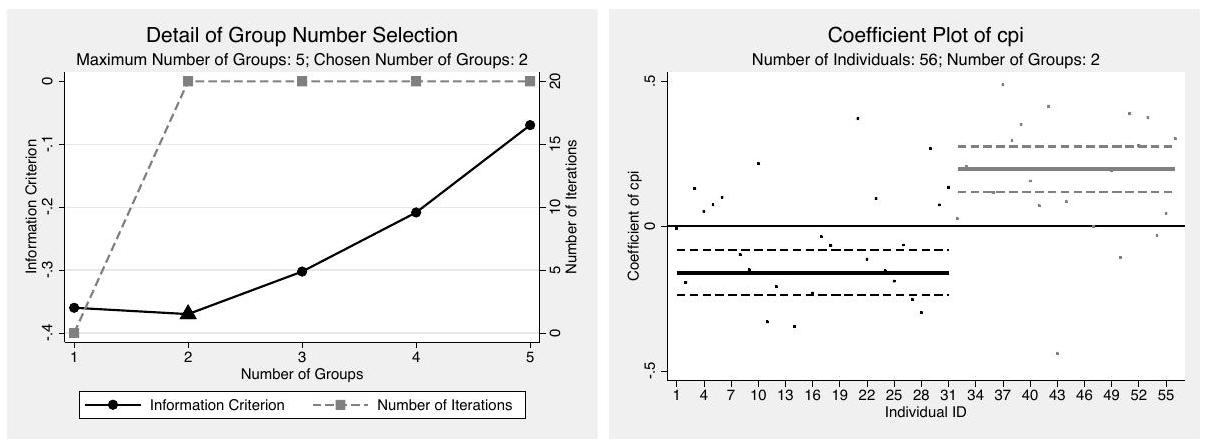
\includegraphics[alt={},max width=\textwidth]{2260cb76-824f-4ec5-b681-a4b165e7b282-15_446_1207_1489_303}
\captionsetup{labelformat=empty}
\caption{Figure 1. Visualization of the implementation example}
\end{center}
\end{figure}

\section*{5 Monte Carlo simulation}
This section evaluates the finite-sample performance of the estimation results generated by the classifylasso command using Monte Carlo simulations. The results are similar to those in Su, Shi, and Phillips (2016), indicating that the command works well.

We consider linear static panels with latent group structures. We consider sample size $N \in\{100,200\}$, time span $T \in\{20,40\}$, and number of covariates $p \in\{2,4\}$. We run 500 replications for each $N, T, p$ combination. The observations in each datagenerating process (DGP) are drawn from three groups with proportion $N_{1}: N_{2}: N_{3}= 0.3: 0.3: 0.4$. The group membership is random against the identity code. The idiosyncratic errors $u_{i t}$ and the fixed effects $\mu_{i}$ follow independent standard normal distributions.

The exogenous regressors are $\mathbf{x}_{i t}=\left(0.2 \mu_{i}+e_{i t 1}, 0.2 \mu_{i}+e_{i t 2}\right)^{\prime}$ for $p=2$ and $\mathbf{x}_{i t}=\left(0.2 \mu_{i}+e_{i t 1}, 0.2 \mu_{i}+e_{i t 2}, 0.3 \mu_{i}+e_{i t 3}, 0.3 \mu_{i}+e_{i t 4}\right)^{\prime}$ for $p=4$, where $e_{i t j}$ are mutually independent and independent with $\mu_{i}$ and $u_{i t}$. The true coefficients are $\boldsymbol{\alpha}_{1}= (0.4,1.6), \boldsymbol{\alpha}_{2}=(1,1), \boldsymbol{\alpha}_{3}=(1.6,0.4)$ for $p=2$; and $\boldsymbol{\alpha}_{1}=(0.4,1.6,-0.4,-1.6), \boldsymbol{\alpha}_{2}= (1,1,-1,-1), \boldsymbol{\alpha}_{3}=(1.6,0.4,-1.6,-0.4)$ for $p=4$, and $y_{i t}=\mathbf{x}_{i t}^{\prime} \boldsymbol{\alpha}_{k}+\mu_{i}+u_{i t}$ for $i \in G_{k}$.

For the tuning parameters, we use the default values in the command; that is, $c_{\lambda}=0.2$ for $\lambda_{N T}=c_{\lambda} T^{-1 / 3}$ and $c_{\rho}=2 / 3$ for $\rho_{N T}=c_{\rho}(N T)^{-1 / 2}$. By default, the individual fixed effects are absorbed by demeaning. For each DGP, we select the group size from 1 to 5 . The implementation command for two covariates is\\
classifylasso y x1 x2, group(1/5)\\
Table 1 (left) reports the frequency of selecting the number of groups $\widehat{K}=1, \ldots, 5$ when the true number of groups $K=3$. It indicates that the information criterion generates perfect selection of the number of groups when $N$ and $T$ increase. These results demonstrate the usefulness of the information criterion and the robustness of the default $\rho$ value.

Table 1 (right) reports the average computation time of different sample sizes, parameter numbers, and group numbers without parallel computation using 3.20 GHz and 8 kernels CPU. Generally, both the capacity of the computer and the attribute of the dataset will affect the computation time. $N$ and $p$ both quadratically increase the computation time, while $T$ does not significantly influence the computation time. In addition, the effect of $K$ on the computation time is nonproportional. Take $N=100$, $T=40$, and $p=4$, for instance; the command requires 12 minutes on average to choose the number of groups from 1 to 5 . The computation burden mainly comes from the optimization of step 1.2 in section 2.3. Note that there is a tradeoff between estimation accuracy and computation time. The users can set the "iteration" parameters $R_{\text {max }}$ and $\epsilon_{\text {tol }}$ using the options to shorten computation time while maintaining enough estimation accuracy. Besides, after each completion of step 1.2, the command will print a dot.

\begin{table}[h]
\begin{center}
\captionsetup{labelformat=empty}
\caption{Table 1. Selecting the number of groups}
\begin{tabular}{|l|l|l|l|l|l|l|l|l|l|l|l|l|}
\hline
\multirow[b]{2}{*}{N} & \multirow[b]{2}{*}{$T$} & \multirow[b]{2}{*}{$p$} & \multicolumn{5}{|l|}{Frequency of selecting $K$} & \multicolumn{5}{|c|}{Computation time (minutes)} \\
\hline
 &  &  & 1 & 2 & 3 & 4 & 5 & 1 & 2 & 3 & 4 & 5 \\
\hline
100 & 20 & 2 & 0 & 0 & 0.998 & 0.002 & 0 & 0.004 & 0.391 & 0.648 & 0.821 & 1.015 \\
\hline
100 & 40 & 2 & 0 & 0 & 1 & 0 & 0 & 0.010 & 0.601 & 0.900 & 1.052 & 0.735 \\
\hline
100 & 20 & 4 & 0 & 0 & 0.99 & 0.01 & 0 & 0.012 & 1.120 & 1.907 & 2.388 & 2.878 \\
\hline
100 & 40 & 4 & 0 & 0 & 1 & 0 & 0 & 0.039 & 1.582 & 2.261 & 3.009 & 2.145 \\
\hline
200 & 20 & 2 & 0 & 0 & 0.998 & 0.002 & 0 & 0.004 & 0.377 & 0.949 & 2.163 & 2.925 \\
\hline
200 & 40 & 2 & 0 & 0 & 1 & 0 & 0 & 0.008 & 0.432 & 1.117 & 2.662 & 2.182 \\
\hline
200 & 20 & 4 & 0 & 0 & 1 & 0 & 0 & 0.012 & 1.544 & 4.157 & 8.837 & 12.826 \\
\hline
200 & 40 & 4 & 0 & 0 & 1 & 0 & 0 & 0.039 & 1.858 & 4.830 & 12.267 & 14.653 \\
\hline
\end{tabular}
\end{center}
\end{table}

Table 2 reports the performance of the classification of individual units and estimation of the parameters. Column 4 reports the accuracy of individual classification, defined as $1 / N \sum_{k=1}^{K} \sum_{i \in \widehat{G}_{k}} \mathbf{1}\left\{\boldsymbol{\beta}_{i}=\boldsymbol{\alpha}_{k}\right\}$, averaged over 500 replications. Columns 5-7 report the postlasso estimators' root mean squared error (RMSE), bias, and coverage probability of the two-sided $95 \%$ confidence interval, averaged over 500 replications. Analogously to Su, Shi, and Phillips (2016), the performance of $\boldsymbol{\alpha}_{1}=\left(\alpha_{k 1}\right)_{k=1}^{K}$ is reported. Because $\boldsymbol{\alpha}_{1}$ is a $K \times 1$ vector, we averaged over the statistics by their weight $N_{k} / N$. For instance, the coverage is defined as $\sum_{k=1}^{K} N_{k} / N \mathbf{1}\left\{\widehat{\alpha}_{\widehat{G}_{k}, 1}-1.96 \widehat{\sigma}_{k 1} \leq \alpha_{k 1} \leq\right. \left.\widehat{\alpha}_{\widehat{G}_{k}, 1}+1.96 \widehat{\sigma}_{k 1}\right\}$. The performances of the other parameters- $\boldsymbol{\alpha}_{2}, \boldsymbol{\alpha}_{3}$, and $\boldsymbol{\alpha}_{4}$ - are similar. For comparison purposes, the performances of the oracle estimators are reported in columns 8-10. The oracle estimators are estimated using the true group classification $G_{k}$, which is not available in practice. These results indicate that as $T$ increases, the individual units are almost perfectly classified, and the performance of the postlasso estimators approaches that of the oracle estimators. It demonstrates good finite-sample performances of the estimators that the classifylasso command generates.

\begin{table}[h]
\begin{center}
\captionsetup{labelformat=empty}
\caption{Table 2. Classification accuracy and estimation performance of $\alpha_{1}$}
\begin{tabular}{|l|l|l|l|l|l|l|l|l|l|}
\hline
\multirow[b]{2}{*}{N} & \multirow[b]{2}{*}{T} & \multirow[b]{2}{*}{$p$} & \multirow[b]{2}{*}{Classification} & \multicolumn{3}{|c|}{Postlasso} & \multicolumn{3}{|c|}{Oracle} \\
\hline
 &  &  &  & RMSE & Bias & Coverage & RMSE & Bias & Coverage \\
\hline
100 & 20 & 2 & 0.9354 & 0.0446 & 0.0114 & 0.9068 & 0.0383 & -0.0014 & 0.9538 \\
\hline
100 & 40 & 2 & 0.9900 & 0.0274 & 0.0024 & 0.9442 & 0.0266 & 0.0004 & 0.9488 \\
\hline
200 & 20 & 2 & 0.9392 & 0.0321 & 0.0124 & 0.8942 & 0.0266 & 0.0006 & 0.9548 \\
\hline
200 & 40 & 2 & 0.9899 & 0.0195 & 0.0013 & 0.9398 & 0.0189 & -0.0006 & 0.9476 \\
\hline
100 & 20 & 4 & 0.9785 & 0.0417 & 0.0058 & 0.9326 & 0.0391 & 0.0007 & 0.9494 \\
\hline
100 & 40 & 4 & 0.9990 & 0.0275 & 0.0001 & 0.9362 & 0.0274 & -0.0002 & 0.9370 \\
\hline
200 & 20 & 4 & 0.9775 & 0.0298 & 0.0047 & 0.9254 & 0.0276 & -0.0003 & 0.9436 \\
\hline
200 & 40 & 4 & 0.9992 & 0.0193 & -0.0001 & 0.9490 & 0.0192 & -0.0003 & 0.9484 \\
\hline
\end{tabular}
\end{center}
\end{table}

Finally, as we discussed before, the beta-min assumption is crucial for the performance of the classifylasso command. Therefore, we analyze the effect of violation. We stick with the DGP of two covariates, while we substitute the parameters with $\boldsymbol{\alpha}_{1}=(1-C, 1+C), \boldsymbol{\alpha}_{2}=(1,1), \boldsymbol{\alpha}_{3}=(1+C, 1-C)$. A smaller constant $C$ represents a more severe violation of the beta-min assumption. We consider values of $C \in\{0.01,0.1,0.3,0.6\}$.

Table 3 presents the results of group classification and parameter estimation when the beta-min assumption may be violated. Columns $3-6$ display the classification accuracy, which reveals that the performance of the classifylasso method is poor in distinguishing between groups when the group-specific coefficients are only slightly different from each other. Columns 7-10 display the coverage probability of the two-sided $95 \%$ confidence interval. Similarly, the coverage is far below the nominal rate when the value of $C$ is small. Overall, the group classification and parameter estimation results are poor if the beta-min assumption is violated. We recommend that users justify the beta-min assumption by economic theory or statistical tests (for example, Pesaran and Yamagata [2008], Su and Chen [2013], and Ando and Bai [2015]) before using the classifylasso command.

\begin{table}[h]
\begin{center}
\captionsetup{labelformat=empty}
\caption{Table 3. Classification and performance under violation of the beta-min assumption}
\begin{tabular}{|l|l|l|l|l|l|l|l|l|l|}
\hline
\multirow[b]{2}{*}{N} & \multirow[b]{2}{*}{$T$} & \multicolumn{4}{|c|}{Correct classification} & \multicolumn{4}{|c|}{Coverage of $\alpha_{1}$} \\
\hline
 &  & $C=0.01$ & 0.1 & 0.3 & 0.6 & 0.01 & 0.1 & 0.3 & 0.6 \\
\hline
100 & 20 & 0.3997 & 0.4719 & 0.7428 & 0.9354 & 0.2616 & 0.3428 & 0.8026 & 0.9068 \\
\hline
100 & 40 & 0.4019 & 0.5246 & 0.8593 & 0.9900 & 0.3412 & 0.4886 & 0.8644 & 0.9442 \\
\hline
200 & 20 & 0.3808 & 0.4720 & 0.7473 & 0.9392 & 0.1494 & 0.2354 & 0.7596 & 0.8942 \\
\hline
200 & 40 & 0.3815 & 0.5038 & 0.8597 & 0.9899 & 0.1880 & 0.3048 & 0.8146 & 0.9398 \\
\hline
\end{tabular}
\end{center}
\end{table}

\section*{6 An empirical illustration}
In this section, we study whether there is unobserved group heterogeneity in the relationship between democracy and economic growth that is still unaccounted for in the existing literature.

\subsection*{6.1 Motivation and data description}
Whether democracy benefits economic growth has long been debated. Doucouliagos and Ulubaşoğlu (2008) reviewed 84 studies and found that despite the indirect effect of democracy on many indices, its effect on growth is still inconclusive. Although Acemoglu et al. (2019) recently constructed a new measure of democracy and provided evidence to support positive effects of democracy on economic growth, opposite views are supported by some facts, such as the spectacular economic growth in China, the middle-income trap in South America, and chaos after the Arab Spring.

Considering inconclusive results on the effect, both the signs and the magnitudes, of democracy on economic growth found in the literature, we adopt the c-lasso estimation method in this study and allow for potential group heterogeneity on such effects.

We consider Acemoglu et al.'s (2019) specification as follows:


\begin{equation*}
\operatorname{lnPGDP}_{i t}=\beta_{i} \text { Democracy }_{i t}+\sum_{j=1}^{l} \gamma_{i, j} \operatorname{lnPGDP}_{i, t-j}+\mu_{i}+\lambda_{t}+u_{i t} \tag{6}
\end{equation*}


$i$ and $t$ denote the country and time index; the dependent variable $\ln \operatorname{PGDP}_{i t}$ is the logarithm of GDP per capita; the independent variable of interest, Democracy ${ }_{i t}$, is a dummy variable recording whether country $i$ is a democracy at year $t ; \mu_{i}$ and $\lambda_{t}$ are country-level and year fixed effects; $u_{i t}$ is the idiosyncratic error; control variables are the lags of the dependent variable; and $l$ is the maximum number of lags. To obtain robust results, we consider the specifications including $1,2,3$, and 4 lags.

In contrast to the homogeneity assumption, $\beta_{i}$, the coefficient of interest, is allowed to vary across countries because of the underlying group pattern, measuring potentially heterogeneous effects of democracy on economic growth.

The data are stored in democracy.dta, provided with the article files. It is transferred from the original dataset into a balanced one with 98 countries from 1970 to 2010. We first import the data and declare the panel structure:

\begin{verbatim}
- use democracy, clear
- xtset country year
Panel variable: country (strongly balanced)
    Time variable: year, 1970 to 2010
        Delta: 1 unit
\end{verbatim}

\subsection*{6.2 Empirical results}
We first determine the number of groups in (6). The following codes implement groupnumber selection controlling for one lag of lnPGDP, visualize the estimation results, and store the estimation result in democracy1.ster. Note that because lag variables are included in the regression, we correct the dynamic panel bias using the dynamic option. Commands allowing for more control variables are similar.

\begin{verbatim}
. classifylasso lnPGDP Democracy ly1, group(1/5) rho(0.2) a(country year) dynamic
    (output omitted)
- set scheme sj
. classogroup, export("selection2.eps)
. classocoef Democracy, export("coefdem.eps")
- estimates save democracy1, replace
\end{verbatim}

Figure 2 visualizes the estimation results. The left subfigure summarizes the groupnumber selection results. It indicates that two groups are selected considering one lag. The right subfigure plots the effects of democracy on economic growth with the $95 \%$\\
confidence bands based on the postlasso estimation results with dynamic bias correction. With more lag controlled, the selected numbers of breaks are consistently greater than 1 . Therefore, there is evidence that the effects of democracy on growth are heterogeneous across different countries. To keep the results of different control variables consistent, we set the number of groups to be two in the following analyses.

\begin{figure}[h]
\begin{center}
  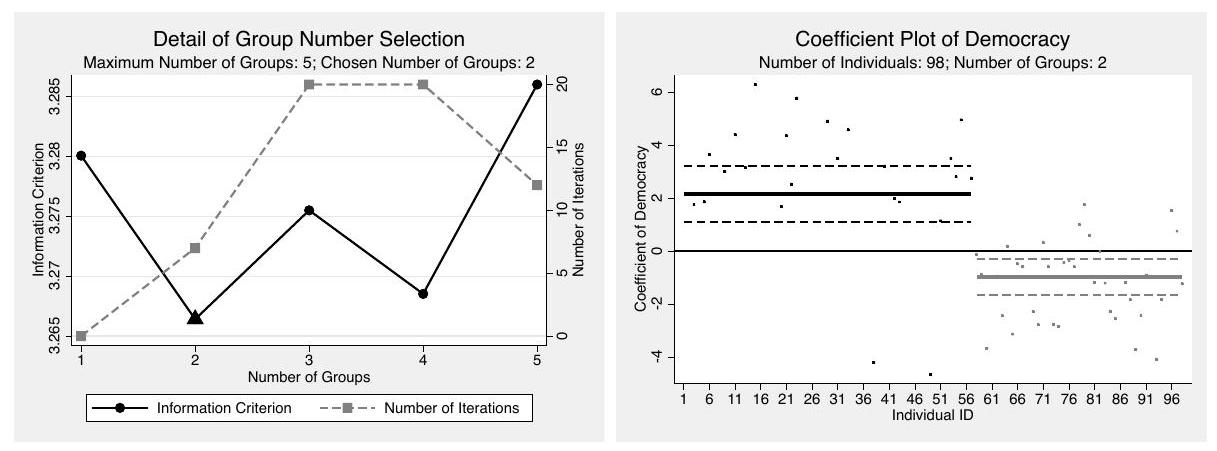
\includegraphics[alt={},max width=\textwidth]{2260cb76-824f-4ec5-b681-a4b165e7b282-20_451_1217_500_296}
\captionsetup{labelformat=empty}
\caption{Figure 2. Heterogeneous effects of democracy on economic growth}
\end{center}
\end{figure}

In what follows, we study the heterogeneous effects of democracy on growth using the c-lasso estimation method and compare them with the original results. The following code implements Acemoglu et al.'s (2019) fixed-effects model estimation and our c-lasso estimation considering both country and year fixed effects. It also stores the coefficients in coeftable.xls.

\begin{verbatim}
- reghdfe lnPGDP Democracy ly1, a(country year) cluster(country)
. outreg2 using "coeftable.xls", replace
\mathrm{ - estimates use democracy1}m
. classoselect, group(2) postselection
. estimates replay, outreg2("coeftable.xls", append)
\end{verbatim}

Table 4 summarizes the estimation results. The four subtables (1), (2), (3), and (4) report the results considering $1,2,3$, and 4 lags, respectively. Within each subtable, the column "Pooled" reports the result of the fixed-effects model. Columns "G1" and "G2" report the postlasso estimation results of two different groups. The clustered standard errors are displayed in the parentheses. $N, T$, and $\#$ obs. are the number of panel units, time periods, and observations, respectively.

\begin{center}
\begin{tabular}{|l|l|l|l|l|l|l|l|l|l|l|l|l|}
\hline
LID＇I & $621^{\prime} 7$ & 979＇ɛ & $907^{\prime} \mathrm{I}$ & $81 \varepsilon^{\prime} 7$ & TZL＇ε & LZG ${ }^{6}$ L & τ0ξ＂ 7 & ζ78＇ɛ & $0 \pm 9^{\prime} \mathrm{I}$ & $08 z^{\prime} z$ & 0z6＇ɛ & ＇sqo \textbackslash ＃ \\
\hline
L\textbackslash ＆ & L\textbackslash ＆ & Σɛ & 88 & 88 & 88 & 68 & 68 & 68 & 0 7 & 0 7 & 0 T & $L$ \\
\hline
I\textbackslash ＆ & 29 & 86 & L\textbackslash ＆ & ［9 & 86 & 68 & 69 & 86 & Lt & 29 & 86 & $N$ \\
\hline
＾ & $\wedge$ & s & ＾ & 1 & ＾ & ＾ & s & s & $\wedge$ & 1 & s & 出 л $^{\text {л }}$ д \\
\hline
（0900） & （gzo．o） & （1z0．0） & $\wedge$ & 1 & ＾ & ＾ & s & s & 1 & 1 & s & ჟу Клашიიე \\
\hline
Z $70^{\circ} 0^{-}$ （890．0） & L700－ （zt0．0） & 970．0－ （L\textbackslash ＆0．0） & （880．0） & （6z0．0） & （2z0．0） &  &  &  &  &  &  & ${ }^{\text {v－}}$ daydut \\
\hline
280.0 （z20．0） & \textbackslash ＆\textbackslash ＆0－ （990．0） & 900．0－ （zgo＇0） & 900．0－ （£20．0） & Z200－ （ $\pounds 90 \cdot 0$ ） & 690．0－ （ $\mathrm{Ig} 0 \%$ ） & （zzł•0） & （ 720.0 ） & （190．0） &  &  &  & ${ }^{\mathcal{E}-}$ dGŋdut \\
\hline
I\textbackslash ＆№－ （990．0） & 0970－ （890．0） & DIZ＇0－ （2900） & 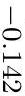
\includegraphics[max width=\textwidth, alt={}]{2260cb76-824f-4ec5-b681-a4b165e7b282-21_96_25_1510_921}
 （2900） & \textbackslash ＆ZO－ （990．0） & 7610－ （990） & τIξ0－ （9z둘） & 2870－ （920．0） & 7870－ （ $z 90 \cdot 0$ ） & （600．0） & （200．0） & （900．0） & ${ }^{\text {z }}$ dGŋduτ \\
\hline
$880^{\circ} \mathrm{I}$ （ $\varepsilon 0 \varepsilon^{\circ} 0$ ） & $\angle \Psi \mathcal{E}^{\circ} \mathrm{I}$ （ειξ＊0） & $877^{\circ} \mathrm{I}$ （ $89 z^{\circ} 0$ ） & \textbackslash ＆\textbackslash ＆IT （ $90 \mathcal{E}^{\circ} 0$ ） & G\textbackslash ＆\textbackslash ＆I （σιξ＊0） & $L Z Z^{\circ} \mathrm{I}$ （69z＇0） & E\textbackslash ＆\textbackslash ＆${ }^{\circ}$ I （ $99 \varepsilon^{\circ} 0$ ） & $60 \varepsilon^{\circ}$ I （ $688^{\circ} 0$ ） & 0971 （ $\varepsilon 9 z \cdot 0$ ） & 7860 （ $87 \mathcal{E}^{\circ} 0$ ） & \textbackslash ＆\textbackslash ＆0＇］ （969．0） & $026^{\circ} 0$ （028．0） & ${ }^{\text {I－}}$ dGŋduτ \\
\hline
ZLI．I－ & $99 \mathrm{I}^{\circ} \mathrm{L}$ & შ78．0 & $797^{\circ} \mathrm{L}$－ & $680^{\circ} \mathrm{I}$ & $892^{\circ} 0$ & 698．0－ & $769^{\circ} \mathrm{I}$ & 182．0 & 186．0－ & 991＇て & $990^{\circ} \mathrm{I}$ & Λაεποοɯθα \\
\hline
75 & ゆ （ t） & рә ${ }^{\circ} \mathrm{OO}_{\mathrm{d}}$ & 25 & ゆ （ɛ） & ／${ }^{\text {月OO }}$ d & 25 & ゆ （Z） & рә $\mathrm{OO}_{\mathrm{d}}$ & 25 & ゆ （I） & рә $\mathrm{OO}_{\mathrm{d}}$ & dGĐduτ \\
\hline
\end{tabular}
\end{center}

\begin{center}
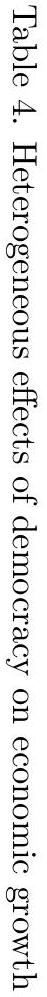
\includegraphics[max width=\textwidth, alt={}]{2260cb76-824f-4ec5-b681-a4b165e7b282-21_997_47_707_1213}
\end{center}

The pooled estimation gives a similar result to the within estimator of table 2 in Acemoglu et al. (2019), indicating that transferring the original dataset into a balanced panel does not influence the core relationship between economic growth and democracy. Postlasso estimation results show consistent polarized effects of democracy on economic growth. Democracy does cause economic growth in countries classified in group 1 (G1), while it hinders economic development and even hurts the economy in those classified in group 2 (G2). Compared with the pooled results, our results uncover group heterogeneity in the effects, which somewhat explains the opposite results found in the literature.

We further analyze the classification results. The results indicate that there are around 60 countries in G1 and around 40 countries in G2. Although the group classification is not completely the same when the number of lags included differs, we find that most disagreement comes from the countries without democratic transitions. ${ }^{1}$

To visualize the heterogeneous effects of democracy on economic growth, we plot the group classification result considering one lag in figure 3. The left subfigure shows all countries in our panel data, and the right one shows countries with a democratic transition. The pale-gray countries are out of our sample. We find that countries such as Korea and Portugal, or South African countries with higher economic development like Zimbabwe, are classified into the group in which democracy promotes growth, while countries classified into the group in which democracy hinders growth include those suffering from civil wars and chaos like Mexico (see Dell [2015]) and those in the poorest region in the world like Zambia, Sudan, and Malawi.

\begin{figure}[h]
\begin{center}
  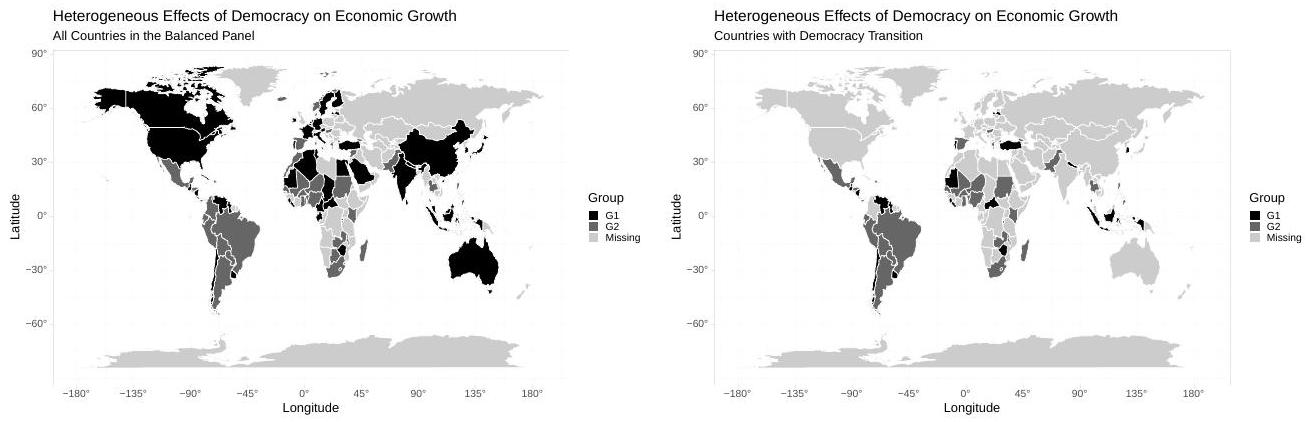
\includegraphics[alt={},max width=\textwidth]{2260cb76-824f-4ec5-b681-a4b165e7b282-22_422_1309_1293_247}
\captionsetup{labelformat=empty}
\caption{Figure 3. Heterogeneous effects of democracy in the world}
\end{center}
\end{figure}

\begin{enumerate}
  \item The democratic transition means that country $i$ was democratic ( Democracy $_{i t}=1, t \in \mathcal{T} \neq \emptyset$ ) at some point in time and nondemocratic at some other point in time ( Democracy $_{i \bar{t}}=0, \bar{t} \in \overline{\mathcal{T}} \neq \emptyset$ ). To obtain a larger dataset, we keep the samples of all countries regardless of whether there is a democratic transition from 1970 to 2010. Results show $73 \%$ of all countries and $76 \%$ of the countries with democratic transitions are consistently classified. Therefore, the main sources of the inconsistent group classification are the countries without democratic transitions.
\end{enumerate}

\section*{7 Conclusions}
In this article, we introduced a new command, classifylasso, that implements the c-lasso method to fit panel-data models with latent group structures in the Stata environment. Postestimation commands are provided to display and visualize the estimation results. The current classifylasso command can be improved in several ways. One possible improvement is to extend the estimation framework to the profile likelihood estimation and the generalized method of moments estimation, as shown in Su, Shi, and Phillips (2016). Another possible improvement is to further speed up the estimation procedure. Although the computation time is acceptable for regular economic datasets, the command may have problems dealing with large financial datasets.

\section*{8 Acknowledgment}
The authors thank the coeditor and the anonymous referee for many constructive comments on the previous version of the article and the command.

\section*{9 Programs and supplemental materials}
To install a snapshot of the corresponding software files as they existed at the time of publication of this article, type

\begin{itemize}
  \item net sj 24-1
  \item net install st0739 (to install program files, if available)
  \item net get st0739 (to install ancillary files, if available)
\end{itemize}

\section*{10 References}
Acemoglu, D., S. Naidu, P. Restrepo, and J. A. Robinson. 2019. Democracy does cause growth. Journal of Political Economy 127: 47-100. \href{https://doi.org/10.1086/700936}{https://doi.org/10.1086/700936}.

Ahrens, A., C. B. Hansen, and M. E. Schaffer. 2020. lassopack: Model selection and prediction with regularized regression in Stata. Stata Journal 20: 176-235. https: // \href{http://doi.org/}{doi.org/} 10.1177/1536867X20909697.

Ahrens, A., C. B. Hansen, M. E. Schaffer, and T. Wiemann. 2024. ddml: Double/debiased machine learning in Stata. Stata Journal 24: 3-45. \href{https://doi.org/10.1177/}{https://doi.org/10.1177/} 1536867 X241233641.

Ando, T., and J. Bai. 2015. A simple new test for slope homogeneity in panel data models with interactive effects. Economics Letters 136: 112-117. https: // \href{http://doi.org}{doi.org} / 10.1016/j.econlet.2015.09.019.

Belloni, A., and V. Chernozhukov. 2013. Least squares after model selection in highdimensional sparse models. Bernoulli 19: 521-547. https: // \href{http://doi.org}{doi.org} / 10.3150 / 11BEJ410.

Belloni, A., V. Chernozhukov, and C. Hansen. 2014. Inference on treatment effects after selection among high-dimensional controls. Review of Economic Studies 81: 608-650. https: // \href{http://doi.org/}{doi.org/} 10.1093/ restud/rdt044.

Bersvendsen, T., and J. Ditzen. 2021. Testing for slope heterogeneity in Stata. Stata Journal 21: 51-80. \href{https://doi.org/10.1177/1536867X211000004}{https://doi.org/10.1177/1536867X211000004}.

Bonhomme, S., and E. Manresa. 2015. Grouped patterns of heterogeneity in panel data. Econometrica 83: 1147-1184. https: // \href{http://doi.org}{doi.org} / 10.3982 / ECTA11319.

Campello, M., A. F. Galvao, and T. Juhl. 2019. Testing for slope heterogeneity bias in panel data models. Journal of Business and Economic Statistics 37: 749-760. https: // \href{http://doi.org/}{doi.org/} 10.1080/ 07350015.2017.1421545.

Carter, A. V., K. T. Schnepel, and D. G. Steigerwald. 2017. Asymptotic behavior of a $t$ test robust to cluster heterogeneity. Review of Economics and Statistics 99: 698-709. \href{https://doi.org/10.1162/REST_a_00639}{https://doi.org/10.1162/REST\_a\_00639}.

Chernozhukov, V., D. Chetverikov, M. Demirer, E. Duflo, C. Hansen, W. Newey, and J. Robins. 2018. Double/debiased machine learning for treatment and structural parameters. Econometrics Journal 21: C1-C68. \href{https://doi.org/10.1111/ectj.12097}{https://doi.org/10.1111/ectj.12097}.

Christodoulou, D., and V. Sarafidis. 2017. Regression clustering for panel-data models with fixed effects. Stata Journal 17: 314-329. https: // \href{http://doi.org}{doi.org} / 10.1177 / 1536867X1701700204.

Correia, S. 2014. reghdfe: Stata module to perform linear or instrumental-variable regression absorbing any number of high-dimensional fixed effects. Statistical Software Components S457874, Department of Economics, Boston College. \href{https://ideas.repec}{https://ideas.repec}. org / c / boc / bocode / s457874.html.\\
\_\_ 2016. ftools: Stata module to provide alternatives to common Stata commands optimized for large datasets. Statistical Software Components S458213, Department of Economics, Boston College. \href{https://ideas.repec.org/c/boc/bocode/s458213.html}{https://ideas.repec.org/c/boc/bocode/s458213.html}.

Dell, M. 2015. Trafficking networks and the Mexican drug war. American Economic Review 105: 1738-1779. \href{https://doi.org/}{https://doi.org/} 10.1257/aer. 20121637.

Dhaene, G., and K. Jochmans. 2015. Split-panel jackknife estimation of fixed-effect models. Review of Economic Studies 82: 991-1030. \href{https://doi.org/10.1093/restud/}{https://doi.org/10.1093/restud/} rdv007.

Doucouliagos, H., and M. A. Ulubaşoğlu. 2008. Democracy and economic growth: A meta-analysis. American Journal of Political Science 52: 61-83. \href{https://doi.org/}{https://doi.org/} 10. 1111/j.1540-5907.2007.00299.x.

Drukker, D. M., and D. Liu. 2022. Finite-sample results for lasso and stepwise Neymanorthogonal Poisson estimators. Econometric Reviews 41: 1047-1076. https: // doi. org / 10.1080/ 07474938.2022.2091363.\\
\_\_ 2023. posw: A command for the stepwise Neyman-orthogonal estimator. Stata Journal 23: 402-417. https:// \href{http://doi.org/10.1177/1536867X231175272}{doi.org/10.1177/1536867X231175272}.

Forthcoming. posis: Stata command for the sure-independence-screening Neyman-orthogonal estimator. Stata Journal.

Du, K. 2017. Econometric convergence test and club clustering using Stata. Stata Journal 17: 882-900. https:// \href{http://doi.org/10.1177/1536867X1801700407}{doi.org/10.1177/1536867X1801700407}.

Eicher, T. S., and A. Leukert. 2009. Institutions and economic performance: Endogeneity and parameter heterogeneity. Journal of Money, Credit and Banking 41: 197-219. https:// \href{http://doi.org/}{doi.org/} 10.1111/j.1538-4616.2008.00193.x.

Gao, Z., and Z. Shi. 2021. Implementing convex optimization in R: Two econometric examples. Computational Economics 58: 1127-1135. \href{https://doi.org/10.1007/s10614-020-09995-z}{https://doi.org/10.1007/s10614-020-09995-z}.

Hirukawa, M., D. Liu, I. Murtazashvili, and A. Prokhorov. 2023. DS-HECK: Doublelasso estimation of Heckman selection model. Empirical Economics 64: 3167-3195. https: // \href{http://doi.org/}{doi.org/} 10.1007/s00181-023-02406-w.

Huang, W., S. Jin, and L. Su. 2020. Identifying latent grouped patterns in cointegrated panels. Econometric Theory 36: 410-456. https: // \href{http://doi.org}{doi.org} / 10.1017 / S0266466619000197.

Lee, C. H., and D. G. Steigerwald. 2018. Inference for clustered data. Stata Journal 18: 447-460. \href{https://doi.org/10.1177/1536867X1801800210}{https://doi.org/10.1177/1536867X1801800210}.

Leeb, H., and B. M. Pötscher. 2005. Model selection and inference: Facts and fiction. Econometric Theory 21: 21-59. https: // \href{http://doi.org}{doi.org} / 10.1017 / S0266466605050036.

\begin{itemize}
  \item 
  \begin{enumerate}
    \setcounter{enumii}{2005}
    \item Can one estimate the conditional distribution of post-model-selection estimators? Annals of Statistics 34: 2554-2591. https: // \href{http://doi.org}{doi.org} / 10.1214 / 009053606000000821.
  \end{enumerate}
\end{itemize}

Lu, X., and L. Su. 2017. Determining the number of groups in latent panel structures with an application to income and democracy. Quantitative Economics 8: 729-760. https: // \href{http://doi.org/}{doi.org/} 10.3982 / QE517.

Pesaran, M. H., and T. Yamagata. 2008. Testing slope homogeneity in large panels. Journal of Econometrics 142: 50-93. \href{https://doi.org/10.1016/j.jeconom.2007.05.010}{https://doi.org/10.1016/j.jeconom.2007.05.010}.

Phillips, P. C. B., and D. Sul. 2007. Transition modeling and econometric convergence tests. Econometrica 75: 1771-1855. \href{https://doi.org/10.1111/j.1468-0262.2007.00811}{https://doi.org/10.1111/j.1468-0262.2007.00811}. x .

Pötscher, B. M., and H. Leeb. 2009. On the distribution of penalized maximum likelihood estimators: The LASSO, SCAD, and thresholding. Journal of Multivariate Analysis 100: 2065-2082. https:// \href{http://doi.org/10.1016/j.jmva.2009.06.010}{doi.org/10.1016/j.jmva.2009.06.010}.

Qian, J., and L. Su. 2016. Shrinkage estimation of common breaks in panel data models via adaptive group fused Lasso. Journal of Econometrics 191: 86-109. https: // doi. org / 10.1016 / j.jeconom.2015.09.004.

Sarafidis, V., and N. Weber. 2015. A partially heterogeneous framework for analyzing panel data. Oxford Bulletin of Economics and Statistics 77: 274-296. https: // doi. org / 10.1111/obes. 12062.

Su, L., and Q. Chen. 2013. Testing homogeneity in panel data models with interactive fixed effects. Econometric Theory 29: 1079-1135. https: // \href{http://doi.org}{doi.org} / 10.1017 / S0266466613000017.

Su, L., Z. Shi, and P. C. B. Phillips. 2016. Identifying latent structures in panel data. Econometrica 84: 2215-2264. https: // \href{http://doi.org/10.3982/ECTA12560}{doi.org/10.3982/ECTA12560}.

Wada, R. 2005. outreg2: Stata module to arrange regression outputs into an illustrative table. Statistical Software Components S456416, Department of Economics, Boston College. \href{https://ideas.repec.org/c/boc/bocode/s456416.html}{https://ideas.repec.org/c/boc/bocode/s456416.html}.

\section*{About the authors}
Wenxin Huang is an associate professor in the Department of Economics at Antai College of Economics and Management, Shanghai Jiao Tong University.\\
Yiru Wang is an assistant professor in the Department of Economics at the University of Pittsburgh.\\
Lingyun Zhou is a PhD student in PBC School of Finance at Tsinghua University.


\end{document}